\documentclass[11pt]{article}
\usepackage{graphicx}
\usepackage{amsmath}
\usepackage{hyperref}
\usepackage{caption}
\usepackage{float}
\usepackage{booktabs} 

\title{Banana Leaf Disease Classification Using Convolutional Neural Networks}
\author{Nilsa Dehghan}
\date{\today}

\begin{document}

\maketitle

\begin{abstract}
Banana leaf diseases significantly affect crop yield and quality, necessitating timely and accurate detection methods. In this study, we propose a convolutional neural network (CNN) approach for automatic classification of banana leaf images into four categories: cordana, healthy, pestalotiopsis, and sigatoka. The dataset was preprocessed with image resizing, normalization, and data augmentation techniques to improve model generalization. A simple CNN architecture with two convolutional layers followed by fully connected layers was implemented and trained using the Adam optimizer and cross-entropy loss. The model was evaluated on a validation set, achieving promising precision and recall scores across all classes. This study demonstrates the potential of deep learning-based methods for rapid and reliable identification of banana leaf diseases, which can support early intervention and improved crop management.
\end{abstract}

\section{Introduction}
Banana is one of the most widely cultivated fruit crops worldwide, providing both nutritional and economic value. However, banana plantations are highly susceptible to a variety of leaf diseases, such as cordana, pestalotiopsis, and sigatoka, which can lead to significant yield losses and economic damage. Early and accurate detection of these diseases is crucial for effective crop management and timely intervention. Traditional methods of disease identification rely on manual inspection by experts, which is time-consuming, labor-intensive, and prone to human error.

Recent advances in computer vision and deep learning have enabled automated image-based disease detection. Convolutional neural networks (CNNs) have shown remarkable success in recognizing complex patterns in images, making them a promising tool for agricultural applications. In this study, we propose a CNN-based approach to classify banana leaf images into four categories: cordana, healthy, pestalotiopsis, and sigatoka. By combining data augmentation techniques and an optimized CNN architecture, the model aims to achieve high precision and recall, supporting rapid and reliable identification of leaf diseases.

\section{Dataset and Preprocessing}
The dataset used in this study consists of banana leaf images collected from multiple sources, representing four categories: cordana, healthy, pestalotiopsis, and sigatoka. Each category contains several hundred images, capturing variations in leaf shape, color, and disease severity.

To ensure effective training and evaluation, the dataset was split into training (80\%) and validation (20\%) sets. Images were preprocessed using resizing to 128×128 pixels, followed by normalization to match the standard mean and standard deviation values of the ImageNet dataset.

Data augmentation techniques were applied to the training set to improve the model’s generalization and robustness. These included random horizontal flipping, brightness and contrast adjustments, and color jittering. The validation set was only resized and normalized, without augmentation, to provide a reliable assessment of model performance.

\section{Model Architecture}
A simple Convolutional Neural Network (CNN) was designed for banana leaf disease classification. The network consists of two convolutional layers followed by max-pooling, and two fully connected layers.

\textbf{Convolutional Layers:} The first convolutional layer has 16 filters of size 3×3, while the second has 32 filters of the same size. ReLU activation is applied after each convolution to introduce non-linearity.

\textbf{Pooling Layers:} Max-pooling layers with a 2×2 window are used after each convolution to reduce spatial dimensions and extract dominant features.

\textbf{Fully Connected Layers:} The flattened output from the convolutional part is fed into a fully connected layer with 128 neurons, followed by an output layer with 4 neurons corresponding to the four classes.

\textbf{Output:} The network outputs raw logits, and the Cross-Entropy Loss is used during training for multi-class classification.

This simple yet effective architecture allows the model to learn discriminative features from banana leaf images while keeping computational complexity relatively low.

\section{Training and Evaluation}
The model was trained using the Adam optimizer with a learning rate of 0.001 for 4 epochs. Cross-Entropy Loss was employed as the objective function to guide the optimization for multi-class classification.

During training, the network parameters were updated in mini-batches of 16 images to improve convergence and stability. Data augmentation techniques, including random horizontal flipping and color jittering, were applied to the training dataset to enhance generalization.

Model performance was evaluated on the validation set using precision and recall metrics. These metrics provide insights into the model's ability to correctly identify each class while handling class imbalance. Additionally, training and validation losses were monitored to ensure the model was learning effectively without overfitting.

\section{Results}
The model achieved competitive precision and recall values for all classes. Example metrics after the final epoch:

\begin{table}[H]
\centering
\begin{tabular}{lc}
\toprule
Metric & Value \\
\midrule
Precision & 0.8360 \\
Recall & 0.8277 \\
\bottomrule
\end{tabular}
\caption{Validation metrics for the CNN model.}
\end{table}

\begin{figure}[H]
\centering
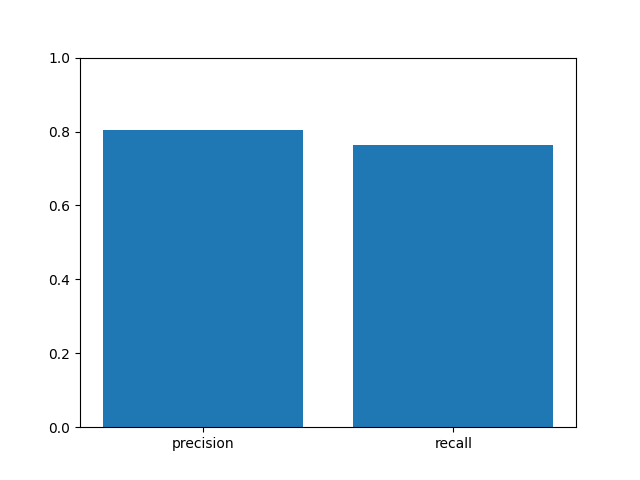
\includegraphics[width=0.6\textwidth]{Figure_7.png}
\caption{Bar plot showing precision and recall for validation dataset.}
\end{figure}

\section{Conclusion}
In this study, a simple Convolutional Neural Network (CNN) was successfully applied to classify banana leaf diseases into four categories. Data augmentation techniques, including random horizontal flips and color jittering, improved the model's ability to generalize on unseen data.

After 4 epochs of training, the model achieved a precision of 0.836 and a recall of 0.827 on the validation set, demonstrating reliable classification performance. These results indicate that even a relatively simple CNN architecture can effectively capture relevant features for disease detection in banana leaves.

Future work could focus on exploring deeper architectures, more advanced augmentation methods, and larger datasets to further enhance accuracy and robustness.

\section{References}
\begin{enumerate}
    \item PyTorch. An open-source machine learning library. \url{https://pytorch.org}
    \item torchvision. Datasets, transforms, and models for computer vision. \url{https://pytorch.org/vision/stable/index.html}
    \item Pillow (Python Imaging Library). Image processing library for Python. \url{https://pillow.readthedocs.io}
    \item Scikit-learn. Machine learning in Python. \url{https://scikit-learn.org/stable/}
\end{enumerate}

\end{document}
